\documentclass{article}\usepackage[]{graphicx}\usepackage[]{color}
% maxwidth is the original width if it is less than linewidth
% otherwise use linewidth (to make sure the graphics do not exceed the margin)
\makeatletter
\def\maxwidth{ %
  \ifdim\Gin@nat@width>\linewidth
    \linewidth
  \else
    \Gin@nat@width
  \fi
}
\makeatother

\definecolor{fgcolor}{rgb}{0.345, 0.345, 0.345}
\newcommand{\hlnum}[1]{\textcolor[rgb]{0.686,0.059,0.569}{#1}}%
\newcommand{\hlstr}[1]{\textcolor[rgb]{0.192,0.494,0.8}{#1}}%
\newcommand{\hlcom}[1]{\textcolor[rgb]{0.678,0.584,0.686}{\textit{#1}}}%
\newcommand{\hlopt}[1]{\textcolor[rgb]{0,0,0}{#1}}%
\newcommand{\hlstd}[1]{\textcolor[rgb]{0.345,0.345,0.345}{#1}}%
\newcommand{\hlkwa}[1]{\textcolor[rgb]{0.161,0.373,0.58}{\textbf{#1}}}%
\newcommand{\hlkwb}[1]{\textcolor[rgb]{0.69,0.353,0.396}{#1}}%
\newcommand{\hlkwc}[1]{\textcolor[rgb]{0.333,0.667,0.333}{#1}}%
\newcommand{\hlkwd}[1]{\textcolor[rgb]{0.737,0.353,0.396}{\textbf{#1}}}%
\let\hlipl\hlkwb

\usepackage{framed}
\makeatletter
\newenvironment{kframe}{%
 \def\at@end@of@kframe{}%
 \ifinner\ifhmode%
  \def\at@end@of@kframe{\end{minipage}}%
  \begin{minipage}{\columnwidth}%
 \fi\fi%
 \def\FrameCommand##1{\hskip\@totalleftmargin \hskip-\fboxsep
 \colorbox{shadecolor}{##1}\hskip-\fboxsep
     % There is no \\@totalrightmargin, so:
     \hskip-\linewidth \hskip-\@totalleftmargin \hskip\columnwidth}%
 \MakeFramed {\advance\hsize-\width
   \@totalleftmargin\z@ \linewidth\hsize
   \@setminipage}}%
 {\par\unskip\endMakeFramed%
 \at@end@of@kframe}
\makeatother

\definecolor{shadecolor}{rgb}{.97, .97, .97}
\definecolor{messagecolor}{rgb}{0, 0, 0}
\definecolor{warningcolor}{rgb}{1, 0, 1}
\definecolor{errorcolor}{rgb}{1, 0, 0}
\newenvironment{knitrout}{}{} % an empty environment to be redefined in TeX

\usepackage{alltt}
\PassOptionsToPackage{unicode}{hyperref}
\PassOptionsToPackage{naturalnames}{hyperref}
\usepackage{fullpage}
\usepackage[T2A]{fontenc}
\usepackage[utf8]{inputenc}
\usepackage[russian]{babel}
\usepackage{mathrsfs}
\usepackage{amsfonts}
\usepackage{amsmath }
\IfFileExists{upquote.sty}{\usepackage{upquote}}{}
\begin{document}
\title{Отчет по домашнему заданию}
\pretitle{\vspace{\droptitle}\centering\huge}
\posttitle{\par}
\author{Фахртдинов Т. А.}


\maketitle
Первая задача. Описательная статистика и проверка гипотезы согласия.

3 вариант.

1) Моделируем величину выигрыша в 50-ти кратном повторении эксперимента, с начальными данными:

$a$ = 10, $b$ = 10, $d$ = 100, $p$ = 0.5, $N$ = 50, $NN$ = 30.

\begin{knitrout}
\definecolor{shadecolor}{rgb}{0.969, 0.969, 0.969}\color{fgcolor}\begin{kframe}
\begin{alltt}
\hlstd{n} \hlkwb{<-} \hlnum{50}
\hlstd{nn} \hlkwb{<-} \hlnum{30}
\hlstd{d} \hlkwb{<-} \hlnum{100}
\hlkwa{for} \hlstd{(i} \hlkwa{in} \hlnum{1} \hlopt{:} \hlstd{n) \{}
  \hlstd{x} \hlkwb{<-} \hlkwd{sample}\hlstd{(}\hlkwd{c}\hlstd{(}\hlnum{10}\hlstd{,}\hlopt{-}\hlnum{10}\hlstd{), n,} \hlkwc{replace}\hlstd{=T,} \hlkwc{prob}\hlstd{=}\hlkwd{c}\hlstd{(}\hlnum{0.5}\hlstd{,} \hlnum{0.5}\hlstd{))}
  \hlstd{res} \hlkwb{<-} \hlkwd{c}\hlstd{(res,} \hlkwd{sum}\hlstd{(x))}
\hlstd{\}}
\hlstd{res} \hlkwb{<-} \hlkwd{as.numeric}\hlstd{(res)}
\hlstd{res}
\end{alltt}
\begin{verbatim}
##  [1]  100   40   60   40   20   40  100  -40   80  -20   40  -40  100 -100  -60
## [16]  -80  -40   60   20   20   20  -80    0  -20  -40  -20    0  -80   60  -40
## [31]  -60   20   40  -40 -100  -20   80  -60  120 -100 -140  -80 -120  -20    0
## [46]  -40   80 -100  -20  -60
\end{verbatim}
\end{kframe}
\end{knitrout}
Берем выборку:
\begin{knitrout}
\definecolor{shadecolor}{rgb}{0.969, 0.969, 0.969}\color{fgcolor}\begin{kframe}
\begin{alltt}
\hlstd{res_sample} \hlkwb{<-} \hlstd{res[}\hlnum{1}\hlopt{:}\hlstd{nn]}
\end{alltt}
\end{kframe}
\end{knitrout}
2) С помощью встроенных функций считаем выборочное среднее (mean) и выборочную дисперсию (var). 

Среднее = 0

Выборочное среднее = 
\begin{knitrout}
\definecolor{shadecolor}{rgb}{0.969, 0.969, 0.969}\color{fgcolor}\begin{kframe}
\begin{verbatim}
## [1] 4.666667
\end{verbatim}
\end{kframe}
\end{knitrout}
Дисперсия = 5000

Выборочная дисперсия = 
\begin{knitrout}
\definecolor{shadecolor}{rgb}{0.969, 0.969, 0.969}\color{fgcolor}\begin{kframe}
\begin{verbatim}
## [1] 3329.195
\end{verbatim}
\end{kframe}
\end{knitrout}
\newpage

3) Посчитать вероятность того, что проигрыш больше d. Посчитать вероятность того, что выигрыш больше d. Посчитать вероятность того, что выигрыш в промежутке от (-d/2; d/2).

Считаем нужные нам вероятности при помощи встроенных функций:

\begin{knitrout}
\definecolor{shadecolor}{rgb}{0.969, 0.969, 0.969}\color{fgcolor}\begin{kframe}
\begin{alltt}
\hlstd{prop_loss_gtd} \hlkwb{<-} \hlkwd{pnorm}\hlstd{(}\hlopt{-}\hlstd{d,} \hlkwc{mean} \hlstd{= mean_res,} \hlkwc{sd} \hlstd{= sd_res_sample)}
\hlstd{prop_win_gtd} \hlkwb{<-} \hlnum{1} \hlopt{-} \hlkwd{pnorm}\hlstd{(d,} \hlkwc{mean} \hlstd{= mean_res,} \hlkwc{sd} \hlstd{= sd_res_sample)}
\hlstd{prop_prof_between} \hlkwb{<-} \hlkwd{pnorm}\hlstd{(d}\hlopt{/}\hlnum{2}\hlstd{,} \hlkwc{mean} \hlstd{= mean_res,} \hlkwc{sd} \hlstd{= sd_res_sample)} \hlopt{-}
\hlkwd{pnorm}\hlstd{(}\hlopt{-}\hlstd{d}\hlopt{/}\hlnum{2}\hlstd{,} \hlkwc{mean} \hlstd{= mean_res,} \hlkwc{sd} \hlstd{= sd_res_sample)}
\end{alltt}
\end{kframe}
\end{knitrout}
Получаем вероятность того, что проигрыш больше d = 
\begin{knitrout}
\definecolor{shadecolor}{rgb}{0.969, 0.969, 0.969}\color{fgcolor}\begin{kframe}
\begin{verbatim}
## [1] 0.05858696
\end{verbatim}
\end{kframe}
\end{knitrout}
Получаем вероятность того, что выигрыш больше d = 
\begin{knitrout}
\definecolor{shadecolor}{rgb}{0.969, 0.969, 0.969}\color{fgcolor}\begin{kframe}
\begin{verbatim}
## [1] 0.02874892
\end{verbatim}
\end{kframe}
\end{knitrout}
Получаем вероятность того, что выигрыш в промежутке от (-d/2; d/2) = 
\begin{knitrout}
\definecolor{shadecolor}{rgb}{0.969, 0.969, 0.969}\color{fgcolor}\begin{kframe}
\begin{verbatim}
## [1] 0.6072784
\end{verbatim}
\end{kframe}
\end{knitrout}
\newpage

4) Строим гистограмму и функцию выборочного распределения:

\begin{knitrout}
\definecolor{shadecolor}{rgb}{0.969, 0.969, 0.969}\color{fgcolor}
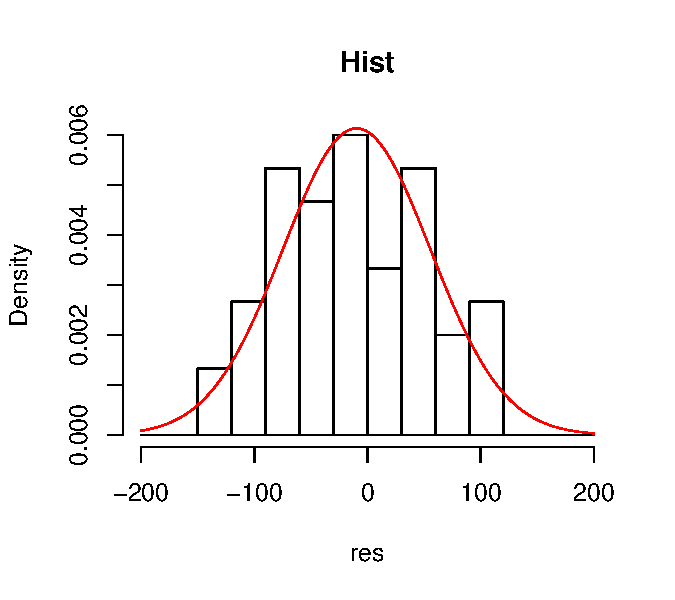
\includegraphics[width=\maxwidth]{figure/unnamed-chunk-12-1} 

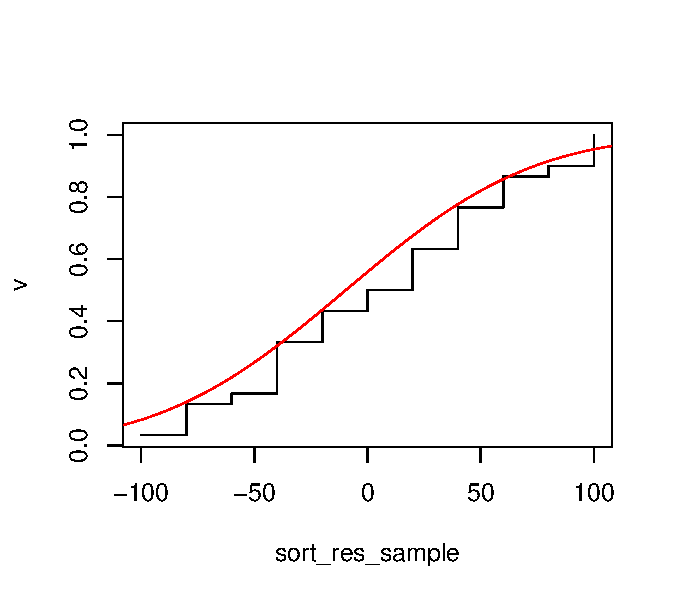
\includegraphics[width=\maxwidth]{figure/unnamed-chunk-12-2} 

\end{knitrout}

\newpage

5) С помощью статистики Пирсона проверяем гипотезу согласия эмпирического распределения с нормальным.
Математическое ожидание моей случайной величины, вычисленное теоретически = 0, дисперсия = 5000. 

$H_0$: Эмпирическое распределение совпадает с распределением $N(0, 5000)$


Возьмем r = 8. Для пункта а) (параметры распределения вычисленны теоретически) посчитаем вектор вероятностей p.

\begin{knitrout}
\definecolor{shadecolor}{rgb}{0.969, 0.969, 0.969}\color{fgcolor}\begin{kframe}
\begin{alltt}
\hlstd{p} \hlkwb{=} \hlkwd{numeric}\hlstd{()}
\hlstd{p} \hlkwb{<-}  \hlkwd{c}\hlstd{(p,} \hlkwd{pnorm}\hlstd{(}\hlopt{-}\hlnum{90}\hlstd{,} \hlkwc{mean} \hlstd{=} \hlnum{0}\hlstd{,} \hlkwc{sd} \hlstd{=} \hlkwd{sqrt}\hlstd{(}\hlnum{5000}\hlstd{))} \hlopt{-}
    \hlkwd{pnorm}\hlstd{(}\hlopt{-}\hlnum{9000}\hlstd{,} \hlkwc{mean} \hlstd{=} \hlnum{0}\hlstd{,} \hlkwc{sd} \hlstd{=} \hlkwd{sqrt}\hlstd{(}\hlnum{5000}\hlstd{)))}
\hlstd{p} \hlkwb{<-} \hlkwd{c}\hlstd{(p,} \hlkwd{pnorm}\hlstd{(}\hlopt{-}\hlnum{55}\hlstd{,} \hlkwc{mean} \hlstd{=} \hlnum{0}\hlstd{,} \hlkwc{sd} \hlstd{=} \hlkwd{sqrt}\hlstd{(}\hlnum{5000}\hlstd{))} \hlopt{-}
           \hlkwd{pnorm}\hlstd{(}\hlopt{-}\hlnum{90}\hlstd{,} \hlkwc{mean} \hlstd{=} \hlnum{0}\hlstd{,} \hlkwc{sd} \hlstd{=} \hlkwd{sqrt}\hlstd{(}\hlnum{5000}\hlstd{)))}
\hlstd{p} \hlkwb{<-} \hlkwd{c}\hlstd{(p,} \hlkwd{pnorm}\hlstd{(}\hlopt{-}\hlnum{30}\hlstd{,} \hlkwc{mean} \hlstd{=} \hlnum{0}\hlstd{,} \hlkwc{sd} \hlstd{=} \hlkwd{sqrt}\hlstd{(}\hlnum{5000}\hlstd{))} \hlopt{-}
           \hlkwd{pnorm}\hlstd{(}\hlopt{-}\hlnum{55}\hlstd{,} \hlkwc{mean} \hlstd{=} \hlnum{0}\hlstd{,} \hlkwc{sd} \hlstd{=} \hlkwd{sqrt}\hlstd{(}\hlnum{5000}\hlstd{)))}
\hlstd{p} \hlkwb{<-} \hlkwd{c}\hlstd{(p,} \hlkwd{pnorm}\hlstd{(}\hlnum{0}\hlstd{,} \hlkwc{mean} \hlstd{=} \hlnum{0}\hlstd{,} \hlkwc{sd} \hlstd{=} \hlkwd{sqrt}\hlstd{(}\hlnum{5000}\hlstd{))} \hlopt{-}
           \hlkwd{pnorm}\hlstd{(}\hlopt{-}\hlnum{30}\hlstd{,} \hlkwc{mean} \hlstd{=} \hlnum{0}\hlstd{,} \hlkwc{sd} \hlstd{=} \hlkwd{sqrt}\hlstd{(}\hlnum{5000}\hlstd{)))}
\hlstd{p} \hlkwb{<-} \hlkwd{c}\hlstd{(p,} \hlkwd{pnorm}\hlstd{(}\hlnum{30}\hlstd{,} \hlkwc{mean} \hlstd{=} \hlnum{0}\hlstd{,} \hlkwc{sd} \hlstd{=} \hlkwd{sqrt}\hlstd{(}\hlnum{5000}\hlstd{))} \hlopt{-}
           \hlkwd{pnorm}\hlstd{(}\hlnum{0}\hlstd{,} \hlkwc{mean} \hlstd{=} \hlnum{0}\hlstd{,} \hlkwc{sd} \hlstd{=} \hlkwd{sqrt}\hlstd{(}\hlnum{5000}\hlstd{)))}
\hlstd{p} \hlkwb{<-} \hlkwd{c}\hlstd{(p,} \hlkwd{pnorm}\hlstd{(}\hlnum{55}\hlstd{,} \hlkwc{mean} \hlstd{=} \hlnum{0}\hlstd{,} \hlkwc{sd} \hlstd{=} \hlkwd{sqrt}\hlstd{(}\hlnum{5000}\hlstd{))} \hlopt{-}
           \hlkwd{pnorm}\hlstd{(}\hlnum{30}\hlstd{,} \hlkwc{mean} \hlstd{=} \hlnum{0}\hlstd{,} \hlkwc{sd} \hlstd{=} \hlkwd{sqrt}\hlstd{(}\hlnum{5000}\hlstd{)))}
\hlstd{p} \hlkwb{<-} \hlkwd{c}\hlstd{(p,} \hlkwd{pnorm}\hlstd{(}\hlnum{90}\hlstd{,} \hlkwc{mean} \hlstd{=} \hlnum{0}\hlstd{,} \hlkwc{sd} \hlstd{=} \hlkwd{sqrt}\hlstd{(}\hlnum{5000}\hlstd{))} \hlopt{-}
           \hlkwd{pnorm}\hlstd{(}\hlnum{55}\hlstd{,} \hlkwc{mean} \hlstd{=} \hlnum{0}\hlstd{,} \hlkwc{sd} \hlstd{=} \hlkwd{sqrt}\hlstd{(}\hlnum{5000}\hlstd{)))}
\hlstd{p} \hlkwb{<-} \hlkwd{c}\hlstd{(p,} \hlkwd{pnorm}\hlstd{(}\hlnum{9000}\hlstd{,} \hlkwc{mean} \hlstd{=} \hlnum{0}\hlstd{,} \hlkwc{sd} \hlstd{=} \hlkwd{sqrt}\hlstd{(}\hlnum{5000}\hlstd{))} \hlopt{-}
    \hlkwd{pnorm}\hlstd{(}\hlnum{90}\hlstd{,} \hlkwc{mean} \hlstd{=} \hlnum{0}\hlstd{,} \hlkwc{sd} \hlstd{=} \hlkwd{sqrt}\hlstd{(}\hlnum{5000}\hlstd{)))}
\end{alltt}
\end{kframe}
\end{knitrout}
Убедимся, что $n*p_i > 5$, а сумма $\sum_i p_i = 1$:
\begin{knitrout}
\definecolor{shadecolor}{rgb}{0.969, 0.969, 0.969}\color{fgcolor}\begin{kframe}
\begin{alltt}
\hlstd{n}\hlopt{*}\hlstd{p}
\end{alltt}
\begin{verbatim}
## [1] 5.077295 5.839621 5.867415 8.215669 8.215669 5.867415 5.839621 5.077295
\end{verbatim}
\begin{alltt}
\hlkwd{sum}\hlstd{(p)}
\end{alltt}
\begin{verbatim}
## [1] 1
\end{verbatim}
\begin{alltt}
\hlstd{br} \hlkwb{<-} \hlkwd{c}\hlstd{(}\hlopt{-}\hlnum{9000}\hlstd{,} \hlopt{-}\hlnum{90}\hlstd{,} \hlopt{-}\hlnum{55}\hlstd{,} \hlopt{-}\hlnum{30}\hlstd{,} \hlnum{0}\hlstd{,} \hlnum{30}\hlstd{,} \hlnum{55}\hlstd{,} \hlnum{90}\hlstd{,} \hlnum{9000}\hlstd{)}
\hlstd{resHIS} \hlkwb{<-} \hlkwd{hist}\hlstd{(res,} \hlkwc{breaks} \hlstd{= br,} \hlkwc{plot} \hlstd{=} \hlnum{FALSE}\hlstd{)}
\hlstd{chiSQ} \hlkwb{<-} \hlstd{(resHIS}\hlopt{$}\hlstd{counts} \hlopt{-} \hlstd{n} \hlopt{*} \hlstd{p)}\hlopt{^}\hlnum{2}
\hlkwa{for} \hlstd{(i} \hlkwa{in} \hlnum{1}\hlopt{:}\hlkwd{length}\hlstd{(p)) \{}
  \hlstd{chiSQ[i]} \hlkwb{=} \hlstd{chiSQ[i]} \hlopt{/} \hlstd{(n} \hlopt{*} \hlstd{p[i])}
\hlstd{\}}
\hlstd{chiSQsumm} \hlkwb{<-} \hlkwd{sum}\hlstd{(chiSQ)}
\hlstd{pValPir} \hlkwb{<-} \hlnum{1} \hlopt{-} \hlkwd{pchisq}\hlstd{(chiSQsumm,} \hlnum{7}\hlstd{)}
\end{alltt}
\end{kframe}
\end{knitrout}

В переменной chiSQsumm записанно значение статистики, а переменной pValPir записанно p - value, величины соответсвенно равны:
\begin{knitrout}
\definecolor{shadecolor}{rgb}{0.969, 0.969, 0.969}\color{fgcolor}\begin{kframe}
\begin{alltt}
\hlstd{chiSQsumm}
\end{alltt}
\begin{verbatim}
## [1] 2.880276
\end{verbatim}
\begin{alltt}
\hlstd{pValPir}
\end{alltt}
\begin{verbatim}
## [1] 0.8958524
\end{verbatim}
\end{kframe}
\end{knitrout}
Убедимся, что результат совпадает со значение встроенной функции:
\begin{knitrout}
\definecolor{shadecolor}{rgb}{0.969, 0.969, 0.969}\color{fgcolor}\begin{kframe}
\begin{alltt}
\hlkwd{chisq.test}\hlstd{(resHIS}\hlopt{$}\hlstd{counts,} \hlkwc{p} \hlstd{= p)}
\end{alltt}
\begin{verbatim}
## 
## 	Chi-squared test for given probabilities
## 
## data:  resHIS$counts
## X-squared = 2.8803, df = 7, p-value = 0.8959
\end{verbatim}
\end{kframe}
\end{knitrout}
По полученным данным нет причин отклонить гипотезу.
\newline
\newline
В пункте б) (параметры распределения оцененны по выборке), воспользуемся функцией pearson.test, пакета nortest, чтобы посчитать значение статистики:
\begin{knitrout}
\definecolor{shadecolor}{rgb}{0.969, 0.969, 0.969}\color{fgcolor}\begin{kframe}
\begin{alltt}
\hlkwd{pearson.test}\hlstd{(res,} \hlkwc{n.classes} \hlstd{=} \hlnum{11}\hlstd{)}
\end{alltt}
\begin{verbatim}
## 
## 	Pearson chi-square normality test
## 
## data:  res
## P = 9.4, p-value = 0.3097
\end{verbatim}
\end{kframe}
\end{knitrout}
По полученным данным нет причин отклонить гипотезу.
\newpage
6) Считаем статиcтики:
Медиана = 
\begin{knitrout}
\definecolor{shadecolor}{rgb}{0.969, 0.969, 0.969}\color{fgcolor}\begin{kframe}
\begin{alltt}
\hlstd{median_res_sample} \hlkwb{<-} \hlkwd{median}\hlstd{(res_sample)}
\hlstd{median_res_sample}
\end{alltt}
\begin{verbatim}
## [1] 10
\end{verbatim}
\end{kframe}
\end{knitrout}
Стандартное отклонение = 
\begin{knitrout}
\definecolor{shadecolor}{rgb}{0.969, 0.969, 0.969}\color{fgcolor}\begin{kframe}
\begin{alltt}
\hlstd{sd_res_sample} \hlkwb{=} \hlkwd{sd}\hlstd{(res_sample)}
\hlstd{sd_res_sample}
\end{alltt}
\begin{verbatim}
## [1] 57.69918
\end{verbatim}
\end{kframe}
\end{knitrout}
Коэффицент вариации = 
\begin{knitrout}
\definecolor{shadecolor}{rgb}{0.969, 0.969, 0.969}\color{fgcolor}\begin{kframe}
\begin{alltt}
\hlstd{sd_res_sample} \hlopt{/} \hlstd{mean_res_sample}
\end{alltt}
\begin{verbatim}
## [1] 12.36411
\end{verbatim}
\end{kframe}
\end{knitrout}
Рассеяние = 
\begin{knitrout}
\definecolor{shadecolor}{rgb}{0.969, 0.969, 0.969}\color{fgcolor}\begin{kframe}
\begin{alltt}
\hlstd{var_res_sample} \hlopt{*} \hlstd{mean_res_sample}
\end{alltt}
\begin{verbatim}
## [1] 15536.25
\end{verbatim}
\end{kframe}
\end{knitrout}
Асимметрия = 
\begin{knitrout}
\definecolor{shadecolor}{rgb}{0.969, 0.969, 0.969}\color{fgcolor}\begin{kframe}
\begin{alltt}
\hlstd{skew_res_sample} \hlkwb{<-} \hlkwd{skewness}\hlstd{(res_sample)}
\hlstd{skew_res_sample}
\end{alltt}
\begin{verbatim}
## [1] -0.0004933734
\end{verbatim}
\end{kframe}
\end{knitrout}
Эксцесс = 
\begin{knitrout}
\definecolor{shadecolor}{rgb}{0.969, 0.969, 0.969}\color{fgcolor}\begin{kframe}
\begin{alltt}
\hlstd{kurt_res_sample} \hlkwb{<-} \hlkwd{kurtosis}\hlstd{(res_sample)}
\hlstd{kurt_res_sample}
\end{alltt}
\begin{verbatim}
## [1] 2.018807
\end{verbatim}
\end{kframe}
\end{knitrout}
95\% доверительный интервал = 
\begin{knitrout}
\definecolor{shadecolor}{rgb}{0.969, 0.969, 0.969}\color{fgcolor}\begin{kframe}
\begin{alltt}
\hlstd{dovInt} \hlkwb{<-} \hlkwd{MeanCI}\hlstd{(res_sample)}
\hlcom{#Левая граница}
\hlstd{dovInt[}\hlnum{2}\hlstd{]}
\end{alltt}
\begin{verbatim}
##    lwr.ci 
## -16.87856
\end{verbatim}
\begin{alltt}
\hlcom{#Правая границы}
\hlstd{dovInt[}\hlnum{3}\hlstd{]}
\end{alltt}
\begin{verbatim}
##   upr.ci 
## 26.21189
\end{verbatim}
\end{kframe}
\end{knitrout}

\end{document}
